\documentclass{standalone}
\usepackage{tikz}
\usetikzlibrary{patterns}
\usetikzlibrary{positioning}
\usetikzlibrary{patterns, positioning}
\usetikzlibrary{shapes.misc}
\usepackage[outline]{contour}
\contourlength{1.5pt} 
\usetikzlibrary{calc}
        \usepackage{relsize}
        \tikzset{fontscale/.style = {font=\relsize{#1}}}

\begin{document}
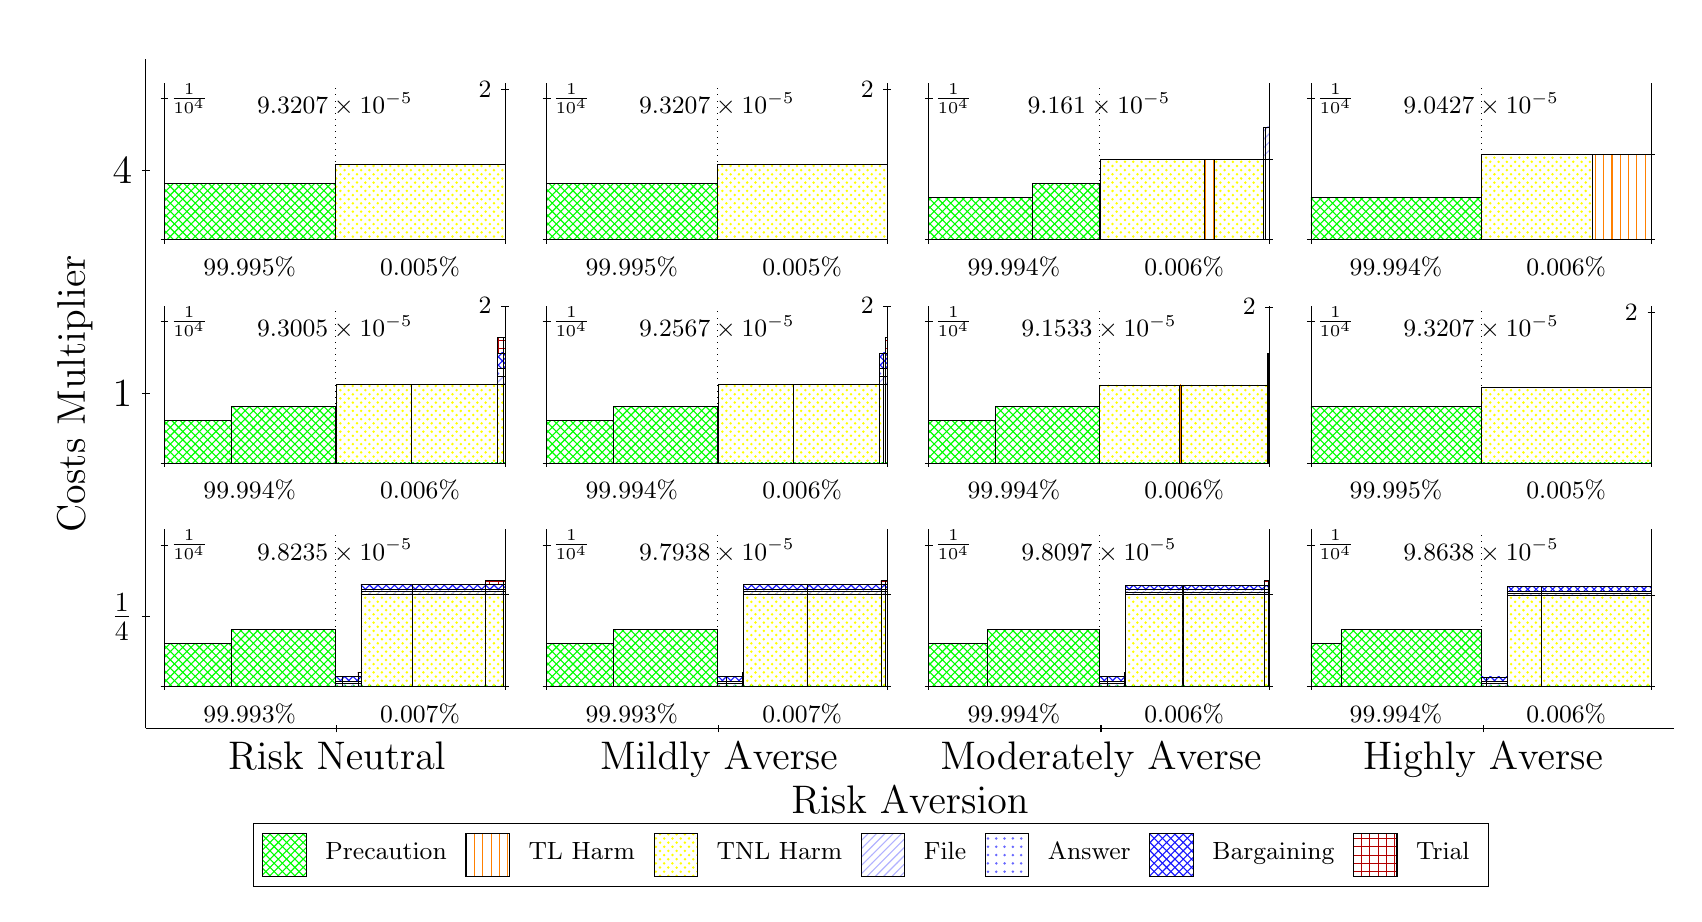
\begin{tikzpicture}
\clip(-0.5,-1.1) rectangle +(20.91,11);
\draw[black] (1,1) -- (1,9.5);
\node[rotate=90, fontscale=2, anchor=center] at (0.1, 5.25) {Costs Multiplier};
\draw[black] (0.95,2.4167) -- (1.05,2.4167);
\node[fontscale=2, anchor=east] at (0.95, 2.4167) {$\frac{1}{4}$};
\draw[black] (0.95,5.25) -- (1.05,5.25);
\node[fontscale=2, anchor=east] at (0.95, 5.25) {1};
\draw[black] (0.95,8.0833) -- (1.05,8.0833);
\node[fontscale=2, anchor=east] at (0.95, 8.0833) {4};

\draw[black] (1,1) -- (20.41,1);
\node[fontscale=2, anchor=center] at (10.705, 0.1) {Risk Aversion};
\draw[black] (3.4263,0.95) -- (3.4263,1.05);
\node[fontscale=2, anchor=north] at (3.4263, 0.95) {Risk Neutral};
\draw[black] (8.2788,0.95) -- (8.2788,1.05);
\node[fontscale=2, anchor=north] at (8.2788, 0.95) {Mildly Averse};
\draw[black] (13.131,0.95) -- (13.131,1.05);
\node[fontscale=2, anchor=north] at (13.131, 0.95) {Moderately Averse};
\draw[black] (17.984,0.95) -- (17.984,1.05);
\node[fontscale=2, anchor=north] at (17.984, 0.95) {Highly Averse};


\draw[pattern=crosshatch, pattern color=green,draw=black,very thin] (1.2381,1.54) rectangle (2.0858,2.0777);
\draw[pattern=crosshatch, pattern color=green,draw=black,very thin] (2.0858,1.54) rectangle (3.4013,2.2569);
\draw[pattern=crosshatch, pattern color=green,draw=black,very thin] (3.4013,1.54) rectangle (3.4917,1.54);
\draw[pattern=north east lines, pattern color=blue!30,draw=black,very thin] (3.4013,1.54) rectangle (3.4917,1.5692);
\draw[pattern=dots,  pattern color=blue!60,draw=black,very thin] (3.4013,1.5692) rectangle (3.4917,1.5985);
\draw[pattern=crosshatch,      pattern color=blue!90,draw=black,very thin] (3.4013,1.5985) rectangle (3.4917,1.6569);
\draw[pattern=crosshatch, pattern color=green,draw=black,very thin] (3.4917,1.54) rectangle (3.6935,1.54);
\draw[pattern=north east lines, pattern color=blue!30,draw=black,very thin] (3.4917,1.54) rectangle (3.6935,1.5693);
\draw[pattern=dots,  pattern color=blue!60,draw=black,very thin] (3.4917,1.5693) rectangle (3.6935,1.5985);
\draw[pattern=crosshatch,      pattern color=blue!90,draw=black,very thin] (3.4917,1.5985) rectangle (3.6935,1.6569);
\draw[pattern=crosshatch, pattern color=green,draw=black,very thin] (3.6935,1.54) rectangle (3.733,1.54);
\draw[pattern=north east lines, pattern color=blue!30,draw=black,very thin] (3.6935,1.54) rectangle (3.733,1.5692);
\draw[pattern=dots,  pattern color=blue!60,draw=black,very thin] (3.6935,1.5692) rectangle (3.733,1.5985);
\draw[pattern=crosshatch,      pattern color=blue!90,draw=black,very thin] (3.6935,1.5985) rectangle (3.733,1.6569);
\draw[pattern=grid,            pattern color=red!70!black,draw=black,very thin] (3.6935,1.6569) rectangle (3.733,1.7153);
\draw[pattern=crosshatch, pattern color=green,draw=black,very thin] (3.733,1.54) rectangle (4.3785,1.54);
\draw[pattern=crosshatch dots, pattern color=yellow,draw=black,very thin] (3.733,1.54) rectangle (4.3785,2.7085);
\draw[pattern=north east lines, pattern color=blue!30,draw=black,very thin] (3.733,2.7085) rectangle (4.3785,2.7378);
\draw[pattern=dots,  pattern color=blue!60,draw=black,very thin] (3.733,2.7378) rectangle (4.3785,2.767);
\draw[pattern=crosshatch,      pattern color=blue!90,draw=black,very thin] (3.733,2.767) rectangle (4.3785,2.8254);
\draw[pattern=crosshatch, pattern color=green,draw=black,very thin] (4.3785,1.54) rectangle (4.38,1.54);
\draw[pattern=vertical lines, pattern color=orange,draw=black,very thin] (4.3785,1.54) rectangle (4.38,2.7085);
\draw[pattern=north east lines, pattern color=blue!30,draw=black,very thin] (4.3785,2.7085) rectangle (4.38,2.7378);
\draw[pattern=dots,  pattern color=blue!60,draw=black,very thin] (4.3785,2.7378) rectangle (4.38,2.767);
\draw[pattern=crosshatch,      pattern color=blue!90,draw=black,very thin] (4.3785,2.767) rectangle (4.38,2.8254);
\draw[pattern=crosshatch, pattern color=green,draw=black,very thin] (4.38,1.54) rectangle (5.3111,1.54);
\draw[pattern=crosshatch dots, pattern color=yellow,draw=black,very thin] (4.38,1.54) rectangle (5.3111,2.7086);
\draw[pattern=north east lines, pattern color=blue!30,draw=black,very thin] (4.38,2.7086) rectangle (5.3111,2.7378);
\draw[pattern=dots,  pattern color=blue!60,draw=black,very thin] (4.38,2.7378) rectangle (5.3111,2.767);
\draw[pattern=crosshatch,      pattern color=blue!90,draw=black,very thin] (4.38,2.767) rectangle (5.3111,2.8254);
\draw[pattern=crosshatch, pattern color=green,draw=black,very thin] (5.3111,1.54) rectangle (5.5362,1.54);
\draw[pattern=crosshatch dots, pattern color=yellow,draw=black,very thin] (5.3111,1.54) rectangle (5.5362,2.7085);
\draw[pattern=north east lines, pattern color=blue!30,draw=black,very thin] (5.3111,2.7085) rectangle (5.5362,2.7378);
\draw[pattern=dots,  pattern color=blue!60,draw=black,very thin] (5.3111,2.7378) rectangle (5.5362,2.767);
\draw[pattern=crosshatch,      pattern color=blue!90,draw=black,very thin] (5.3111,2.767) rectangle (5.5362,2.8254);
\draw[pattern=grid,            pattern color=red!70!black,draw=black,very thin] (5.3111,2.8254) rectangle (5.5362,2.8838);
\draw[pattern=crosshatch, pattern color=green,draw=black,very thin] (5.5362,1.54) rectangle (5.5644,1.54);
\draw[pattern=vertical lines, pattern color=orange,draw=black,very thin] (5.5362,1.54) rectangle (5.5644,2.7085);
\draw[pattern=north east lines, pattern color=blue!30,draw=black,very thin] (5.5362,2.7085) rectangle (5.5644,2.7378);
\draw[pattern=dots,  pattern color=blue!60,draw=black,very thin] (5.5362,2.7378) rectangle (5.5644,2.767);
\draw[pattern=crosshatch,      pattern color=blue!90,draw=black,very thin] (5.5362,2.767) rectangle (5.5644,2.8254);
\draw[pattern=grid,            pattern color=red!70!black,draw=black,very thin] (5.5362,2.8254) rectangle (5.5644,2.8838);
\node[font=\small,text=black,anchor=north] at (3.4013, 3.5333) {$9.8235\times 10^{-5}$};
\draw[black,very thin] (1.2381,1.54) -- (1.2381,3.5333);
\draw[black,very thin] (1.1881,1.54) -- (1.2881,1.54);
\node[font=\small,text=black, anchor=west] at (1.1881, 1.54) {};
\draw[black,very thin] (1.1881,3.3323) -- (1.2881,3.3323);
\node[font=\small,text=black, anchor=west] at (1.1881, 3.3323) {$\frac{1}{10^{4}}$};

\draw[black,dotted,very thin] (3.4013,1.5998) -- (3.4013,3.4735);
\draw[black,very thin] (5.5644,1.54) -- (5.5644,3.5333);
\draw[black,very thin] (5.5144,1.54) -- (5.6144,1.54);
\node[font=\small,text=black, anchor=east] at (5.5144, 1.54) {\contour{white}{}};
\draw[black,very thin] (5.5144,2.7085) -- (5.6144,2.7085);
\node[font=\small,text=black, anchor=east] at (5.5144, 2.7085) {\contour{white}{}};

\draw[black,very thin] (1.2381,1.54) -- (5.5644,1.54);
\draw[black,very thin] (1.2381,1.49) -- (1.2381,1.59);
\node[font=\small,text=black, anchor=north] at (1.2381, 1.49) {};
\draw[black,very thin] (5.5644,1.49) -- (5.5644,1.59);
\node[font=\small,text=black, anchor=north] at (5.5644, 1.49) {};

\node[font=\small,text=black,anchor=south] at (2.3197, 0.94) {99.993\%};
\node[font=\small,text=black,anchor=south] at (4.4828, 0.94) {0.007\%};

\draw[pattern=crosshatch, pattern color=green,draw=black,very thin] (6.0906,1.54) rectangle (6.9383,2.0777);
\draw[pattern=crosshatch, pattern color=green,draw=black,very thin] (6.9383,1.54) rectangle (8.2538,2.2569);
\draw[pattern=crosshatch, pattern color=green,draw=black,very thin] (8.2538,1.54) rectangle (8.3701,1.54);
\draw[pattern=north east lines, pattern color=blue!30,draw=black,very thin] (8.2538,1.54) rectangle (8.3701,1.5692);
\draw[pattern=dots,  pattern color=blue!60,draw=black,very thin] (8.2538,1.5692) rectangle (8.3701,1.5985);
\draw[pattern=crosshatch,      pattern color=blue!90,draw=black,very thin] (8.2538,1.5985) rectangle (8.3701,1.6569);
\draw[pattern=crosshatch, pattern color=green,draw=black,very thin] (8.3701,1.54) rectangle (8.5719,1.54);
\draw[pattern=north east lines, pattern color=blue!30,draw=black,very thin] (8.3701,1.54) rectangle (8.5719,1.5693);
\draw[pattern=dots,  pattern color=blue!60,draw=black,very thin] (8.3701,1.5693) rectangle (8.5719,1.5985);
\draw[pattern=crosshatch,      pattern color=blue!90,draw=black,very thin] (8.3701,1.5985) rectangle (8.5719,1.6569);
\draw[pattern=crosshatch, pattern color=green,draw=black,very thin] (8.5719,1.54) rectangle (8.5856,1.54);
\draw[pattern=north east lines, pattern color=blue!30,draw=black,very thin] (8.5719,1.54) rectangle (8.5856,1.5692);
\draw[pattern=dots,  pattern color=blue!60,draw=black,very thin] (8.5719,1.5692) rectangle (8.5856,1.5985);
\draw[pattern=crosshatch,      pattern color=blue!90,draw=black,very thin] (8.5719,1.5985) rectangle (8.5856,1.6569);
\draw[pattern=grid,            pattern color=red!70!black,draw=black,very thin] (8.5719,1.6569) rectangle (8.5856,1.7153);
\draw[pattern=crosshatch, pattern color=green,draw=black,very thin] (8.5856,1.54) rectangle (9.3953,1.54);
\draw[pattern=crosshatch dots, pattern color=yellow,draw=black,very thin] (8.5856,1.54) rectangle (9.3953,2.7086);
\draw[pattern=north east lines, pattern color=blue!30,draw=black,very thin] (8.5856,2.7086) rectangle (9.3953,2.7378);
\draw[pattern=dots,  pattern color=blue!60,draw=black,very thin] (8.5856,2.7378) rectangle (9.3953,2.767);
\draw[pattern=crosshatch,      pattern color=blue!90,draw=black,very thin] (8.5856,2.767) rectangle (9.3953,2.8254);
\draw[pattern=crosshatch, pattern color=green,draw=black,very thin] (9.3953,1.54) rectangle (9.4038,1.54);
\draw[pattern=vertical lines, pattern color=orange,draw=black,very thin] (9.3953,1.54) rectangle (9.4038,2.7086);
\draw[pattern=north east lines, pattern color=blue!30,draw=black,very thin] (9.3953,2.7086) rectangle (9.4038,2.7378);
\draw[pattern=dots,  pattern color=blue!60,draw=black,very thin] (9.3953,2.7378) rectangle (9.4038,2.767);
\draw[pattern=crosshatch,      pattern color=blue!90,draw=black,very thin] (9.3953,2.767) rectangle (9.4038,2.8254);
\draw[pattern=crosshatch, pattern color=green,draw=black,very thin] (9.4038,1.54) rectangle (10.335,1.54);
\draw[pattern=crosshatch dots, pattern color=yellow,draw=black,very thin] (9.4038,1.54) rectangle (10.335,2.7086);
\draw[pattern=north east lines, pattern color=blue!30,draw=black,very thin] (9.4038,2.7086) rectangle (10.335,2.7378);
\draw[pattern=dots,  pattern color=blue!60,draw=black,very thin] (9.4038,2.7378) rectangle (10.335,2.767);
\draw[pattern=crosshatch,      pattern color=blue!90,draw=black,very thin] (9.4038,2.767) rectangle (10.335,2.8254);
\draw[pattern=crosshatch, pattern color=green,draw=black,very thin] (10.335,1.54) rectangle (10.396,1.54);
\draw[pattern=crosshatch dots, pattern color=yellow,draw=black,very thin] (10.335,1.54) rectangle (10.396,2.7086);
\draw[pattern=north east lines, pattern color=blue!30,draw=black,very thin] (10.335,2.7086) rectangle (10.396,2.7378);
\draw[pattern=dots,  pattern color=blue!60,draw=black,very thin] (10.335,2.7378) rectangle (10.396,2.767);
\draw[pattern=crosshatch,      pattern color=blue!90,draw=black,very thin] (10.335,2.767) rectangle (10.396,2.8254);
\draw[pattern=grid,            pattern color=red!70!black,draw=black,very thin] (10.335,2.8254) rectangle (10.396,2.8838);
\draw[pattern=crosshatch, pattern color=green,draw=black,very thin] (10.396,1.54) rectangle (10.417,1.54);
\draw[pattern=vertical lines, pattern color=orange,draw=black,very thin] (10.396,1.54) rectangle (10.417,2.7086);
\draw[pattern=north east lines, pattern color=blue!30,draw=black,very thin] (10.396,2.7086) rectangle (10.417,2.7378);
\draw[pattern=dots,  pattern color=blue!60,draw=black,very thin] (10.396,2.7378) rectangle (10.417,2.767);
\draw[pattern=crosshatch,      pattern color=blue!90,draw=black,very thin] (10.396,2.767) rectangle (10.417,2.8254);
\draw[pattern=grid,            pattern color=red!70!black,draw=black,very thin] (10.396,2.8254) rectangle (10.417,2.8838);
\node[font=\small,text=black,anchor=north] at (8.2538, 3.5333) {$9.7938\times 10^{-5}$};
\draw[black,very thin] (6.0906,1.54) -- (6.0906,3.5333);
\draw[black,very thin] (6.0406,1.54) -- (6.1406,1.54);
\node[font=\small,text=black, anchor=west] at (6.0406, 1.54) {};
\draw[black,very thin] (6.0406,3.3323) -- (6.1406,3.3323);
\node[font=\small,text=black, anchor=west] at (6.0406, 3.3323) {$\frac{1}{10^{4}}$};

\draw[black,dotted,very thin] (8.2538,1.5998) -- (8.2538,3.4735);
\draw[black,very thin] (10.417,1.54) -- (10.417,3.5333);
\draw[black,very thin] (10.367,1.54) -- (10.467,1.54);
\node[font=\small,text=black, anchor=east] at (10.367, 1.54) {\contour{white}{}};
\draw[black,very thin] (10.367,2.7085) -- (10.467,2.7085);
\node[font=\small,text=black, anchor=east] at (10.367, 2.7085) {\contour{white}{}};

\draw[black,very thin] (6.0906,1.54) -- (10.417,1.54);
\draw[black,very thin] (6.0906,1.49) -- (6.0906,1.59);
\node[font=\small,text=black, anchor=north] at (6.0906, 1.49) {};
\draw[black,very thin] (10.417,1.49) -- (10.417,1.59);
\node[font=\small,text=black, anchor=north] at (10.417, 1.49) {};

\node[font=\small,text=black,anchor=south] at (7.1722, 0.94) {99.993\%};
\node[font=\small,text=black,anchor=south] at (9.3353, 0.94) {0.007\%};

\draw[pattern=crosshatch, pattern color=green,draw=black,very thin] (10.943,1.54) rectangle (11.692,2.0777);
\draw[pattern=crosshatch, pattern color=green,draw=black,very thin] (11.692,1.54) rectangle (13.106,2.2569);
\draw[pattern=crosshatch, pattern color=green,draw=black,very thin] (13.106,1.54) rectangle (13.21,1.54);
\draw[pattern=north east lines, pattern color=blue!30,draw=black,very thin] (13.106,1.54) rectangle (13.21,1.5691);
\draw[pattern=dots,  pattern color=blue!60,draw=black,very thin] (13.106,1.5691) rectangle (13.21,1.5982);
\draw[pattern=crosshatch,      pattern color=blue!90,draw=black,very thin] (13.106,1.5982) rectangle (13.21,1.6564);
\draw[pattern=crosshatch, pattern color=green,draw=black,very thin] (13.21,1.54) rectangle (13.428,1.54);
\draw[pattern=north east lines, pattern color=blue!30,draw=black,very thin] (13.21,1.54) rectangle (13.428,1.5691);
\draw[pattern=dots,  pattern color=blue!60,draw=black,very thin] (13.21,1.5691) rectangle (13.428,1.5982);
\draw[pattern=crosshatch,      pattern color=blue!90,draw=black,very thin] (13.21,1.5982) rectangle (13.428,1.6564);
\draw[pattern=crosshatch, pattern color=green,draw=black,very thin] (13.428,1.54) rectangle (13.439,1.54);
\draw[pattern=north east lines, pattern color=blue!30,draw=black,very thin] (13.428,1.54) rectangle (13.439,1.5691);
\draw[pattern=dots,  pattern color=blue!60,draw=black,very thin] (13.428,1.5691) rectangle (13.439,1.5982);
\draw[pattern=crosshatch,      pattern color=blue!90,draw=black,very thin] (13.428,1.5982) rectangle (13.439,1.6564);
\draw[pattern=grid,            pattern color=red!70!black,draw=black,very thin] (13.428,1.6564) rectangle (13.439,1.7146);
\draw[pattern=crosshatch, pattern color=green,draw=black,very thin] (13.439,1.54) rectangle (14.165,1.54);
\draw[pattern=crosshatch dots, pattern color=yellow,draw=black,very thin] (13.439,1.54) rectangle (14.165,2.7041);
\draw[pattern=north east lines, pattern color=blue!30,draw=black,very thin] (13.439,2.7041) rectangle (14.165,2.7332);
\draw[pattern=dots,  pattern color=blue!60,draw=black,very thin] (13.439,2.7332) rectangle (14.165,2.7623);
\draw[pattern=crosshatch,      pattern color=blue!90,draw=black,very thin] (13.439,2.7623) rectangle (14.165,2.8205);
\draw[pattern=crosshatch, pattern color=green,draw=black,very thin] (14.165,1.54) rectangle (14.171,1.54);
\draw[pattern=vertical lines, pattern color=orange,draw=black,very thin] (14.165,1.54) rectangle (14.171,2.7041);
\draw[pattern=north east lines, pattern color=blue!30,draw=black,very thin] (14.165,2.7041) rectangle (14.171,2.7332);
\draw[pattern=dots,  pattern color=blue!60,draw=black,very thin] (14.165,2.7332) rectangle (14.171,2.7623);
\draw[pattern=crosshatch,      pattern color=blue!90,draw=black,very thin] (14.165,2.7623) rectangle (14.171,2.8205);
\draw[pattern=crosshatch, pattern color=green,draw=black,very thin] (14.171,1.54) rectangle (15.2,1.54);
\draw[pattern=crosshatch dots, pattern color=yellow,draw=black,very thin] (14.171,1.54) rectangle (15.2,2.7041);
\draw[pattern=north east lines, pattern color=blue!30,draw=black,very thin] (14.171,2.7041) rectangle (15.2,2.7332);
\draw[pattern=dots,  pattern color=blue!60,draw=black,very thin] (14.171,2.7332) rectangle (15.2,2.7623);
\draw[pattern=crosshatch,      pattern color=blue!90,draw=black,very thin] (14.171,2.7623) rectangle (15.2,2.8205);
\draw[pattern=crosshatch, pattern color=green,draw=black,very thin] (15.2,1.54) rectangle (15.252,1.54);
\draw[pattern=crosshatch dots, pattern color=yellow,draw=black,very thin] (15.2,1.54) rectangle (15.252,2.7041);
\draw[pattern=north east lines, pattern color=blue!30,draw=black,very thin] (15.2,2.7041) rectangle (15.252,2.7332);
\draw[pattern=dots,  pattern color=blue!60,draw=black,very thin] (15.2,2.7332) rectangle (15.252,2.7623);
\draw[pattern=crosshatch,      pattern color=blue!90,draw=black,very thin] (15.2,2.7623) rectangle (15.252,2.8205);
\draw[pattern=grid,            pattern color=red!70!black,draw=black,very thin] (15.2,2.8205) rectangle (15.252,2.8787);
\draw[pattern=crosshatch, pattern color=green,draw=black,very thin] (15.252,1.54) rectangle (15.269,1.54);
\draw[pattern=vertical lines, pattern color=orange,draw=black,very thin] (15.252,1.54) rectangle (15.269,2.7041);
\draw[pattern=north east lines, pattern color=blue!30,draw=black,very thin] (15.252,2.7041) rectangle (15.269,2.7332);
\draw[pattern=dots,  pattern color=blue!60,draw=black,very thin] (15.252,2.7332) rectangle (15.269,2.7623);
\draw[pattern=crosshatch,      pattern color=blue!90,draw=black,very thin] (15.252,2.7623) rectangle (15.269,2.8205);
\draw[pattern=grid,            pattern color=red!70!black,draw=black,very thin] (15.252,2.8205) rectangle (15.269,2.8787);
\node[font=\small,text=black,anchor=north] at (13.106, 3.5333) {$9.8097\times 10^{-5}$};
\draw[black,very thin] (10.943,1.54) -- (10.943,3.5333);
\draw[black,very thin] (10.893,1.54) -- (10.993,1.54);
\node[font=\small,text=black, anchor=west] at (10.893, 1.54) {};
\draw[black,very thin] (10.893,3.3323) -- (10.993,3.3323);
\node[font=\small,text=black, anchor=west] at (10.893, 3.3323) {$\frac{1}{10^{4}}$};

\draw[black,dotted,very thin] (13.106,1.5998) -- (13.106,3.4735);
\draw[black,very thin] (15.269,1.54) -- (15.269,3.5333);
\draw[black,very thin] (15.219,1.54) -- (15.319,1.54);
\node[font=\small,text=black, anchor=east] at (15.219, 1.54) {\contour{white}{}};
\draw[black,very thin] (15.219,2.704) -- (15.319,2.704);
\node[font=\small,text=black, anchor=east] at (15.219, 2.704) {\contour{white}{}};

\draw[black,very thin] (10.943,1.54) -- (15.269,1.54);
\draw[black,very thin] (10.943,1.49) -- (10.943,1.59);
\node[font=\small,text=black, anchor=north] at (10.943, 1.49) {};
\draw[black,very thin] (15.269,1.49) -- (15.269,1.59);
\node[font=\small,text=black, anchor=north] at (15.269, 1.49) {};

\node[font=\small,text=black,anchor=south] at (12.025, 0.94) {99.994\%};
\node[font=\small,text=black,anchor=south] at (14.188, 0.94) {0.006\%};

\draw[pattern=crosshatch, pattern color=green,draw=black,very thin] (15.796,1.54) rectangle (16.177,2.0777);
\draw[pattern=crosshatch, pattern color=green,draw=black,very thin] (16.177,1.54) rectangle (17.959,2.2569);
\draw[pattern=crosshatch, pattern color=green,draw=black,very thin] (17.959,1.54) rectangle (18.018,1.54);
\draw[pattern=north east lines, pattern color=blue!30,draw=black,very thin] (17.959,1.54) rectangle (18.018,1.5687);
\draw[pattern=dots,  pattern color=blue!60,draw=black,very thin] (17.959,1.5687) rectangle (18.018,1.5974);
\draw[pattern=crosshatch,      pattern color=blue!90,draw=black,very thin] (17.959,1.5974) rectangle (18.018,1.6547);
\draw[pattern=crosshatch, pattern color=green,draw=black,very thin] (18.018,1.54) rectangle (18.297,1.54);
\draw[pattern=north east lines, pattern color=blue!30,draw=black,very thin] (18.018,1.54) rectangle (18.297,1.5687);
\draw[pattern=dots,  pattern color=blue!60,draw=black,very thin] (18.018,1.5687) rectangle (18.297,1.5974);
\draw[pattern=crosshatch,      pattern color=blue!90,draw=black,very thin] (18.018,1.5974) rectangle (18.297,1.6548);
\draw[pattern=crosshatch, pattern color=green,draw=black,very thin] (18.297,1.54) rectangle (18.721,1.54);
\draw[pattern=crosshatch dots, pattern color=yellow,draw=black,very thin] (18.297,1.54) rectangle (18.721,2.6872);
\draw[pattern=north east lines, pattern color=blue!30,draw=black,very thin] (18.297,2.6872) rectangle (18.721,2.7158);
\draw[pattern=dots,  pattern color=blue!60,draw=black,very thin] (18.297,2.7158) rectangle (18.721,2.7445);
\draw[pattern=crosshatch,      pattern color=blue!90,draw=black,very thin] (18.297,2.7445) rectangle (18.721,2.8019);
\draw[pattern=crosshatch, pattern color=green,draw=black,very thin] (18.721,1.54) rectangle (18.723,1.54);
\draw[pattern=vertical lines, pattern color=orange,draw=black,very thin] (18.721,1.54) rectangle (18.723,2.6872);
\draw[pattern=north east lines, pattern color=blue!30,draw=black,very thin] (18.721,2.6872) rectangle (18.723,2.7158);
\draw[pattern=dots,  pattern color=blue!60,draw=black,very thin] (18.721,2.7158) rectangle (18.723,2.7445);
\draw[pattern=crosshatch,      pattern color=blue!90,draw=black,very thin] (18.721,2.7445) rectangle (18.723,2.8019);
\draw[pattern=crosshatch, pattern color=green,draw=black,very thin] (18.723,1.54) rectangle (20.122,1.54);
\draw[pattern=crosshatch dots, pattern color=yellow,draw=black,very thin] (18.723,1.54) rectangle (20.122,2.6872);
\draw[pattern=north east lines, pattern color=blue!30,draw=black,very thin] (18.723,2.6872) rectangle (20.122,2.7158);
\draw[pattern=dots,  pattern color=blue!60,draw=black,very thin] (18.723,2.7158) rectangle (20.122,2.7445);
\draw[pattern=crosshatch,      pattern color=blue!90,draw=black,very thin] (18.723,2.7445) rectangle (20.122,2.8019);
\node[font=\small,text=black,anchor=north] at (17.959, 3.5333) {$9.8638\times 10^{-5}$};
\draw[black,very thin] (15.796,1.54) -- (15.796,3.5333);
\draw[black,very thin] (15.746,1.54) -- (15.846,1.54);
\node[font=\small,text=black, anchor=west] at (15.746, 1.54) {};
\draw[black,very thin] (15.746,3.3323) -- (15.846,3.3323);
\node[font=\small,text=black, anchor=west] at (15.746, 3.3323) {$\frac{1}{10^{4}}$};

\draw[black,dotted,very thin] (17.959,1.5998) -- (17.959,3.4735);
\draw[black,very thin] (20.122,1.54) -- (20.122,3.5333);
\draw[black,very thin] (20.072,1.54) -- (20.172,1.54);
\node[font=\small,text=black, anchor=east] at (20.072, 1.54) {\contour{white}{}};
\draw[black,very thin] (20.072,2.6871) -- (20.172,2.6871);
\node[font=\small,text=black, anchor=east] at (20.072, 2.6871) {\contour{white}{}};

\draw[black,very thin] (15.796,1.54) -- (20.122,1.54);
\draw[black,very thin] (15.796,1.49) -- (15.796,1.59);
\node[font=\small,text=black, anchor=north] at (15.796, 1.49) {};
\draw[black,very thin] (20.122,1.49) -- (20.122,1.59);
\node[font=\small,text=black, anchor=north] at (20.122, 1.49) {};

\node[font=\small,text=black,anchor=south] at (16.877, 0.94) {99.994\%};
\node[font=\small,text=black,anchor=south] at (19.04, 0.94) {0.006\%};

\draw[pattern=crosshatch, pattern color=green,draw=black,very thin] (1.2381,4.3733) rectangle (2.0858,4.911);
\draw[pattern=crosshatch, pattern color=green,draw=black,very thin] (2.0858,4.3733) rectangle (3.4013,5.0903);
\draw[pattern=crosshatch, pattern color=green,draw=black,very thin] (3.4013,4.3733) rectangle (3.4172,4.3734);
\draw[pattern=north east lines, pattern color=blue!30,draw=black,very thin] (3.4013,4.3734) rectangle (3.4172,4.473);
\draw[pattern=dots,  pattern color=blue!60,draw=black,very thin] (3.4013,4.473) rectangle (3.4172,4.5727);
\draw[pattern=crosshatch,      pattern color=blue!90,draw=black,very thin] (3.4013,4.5727) rectangle (3.4172,4.772);
\draw[pattern=grid,            pattern color=red!70!black,draw=black,very thin] (3.4013,4.772) rectangle (3.4172,4.9714);
\draw[pattern=crosshatch, pattern color=green,draw=black,very thin] (3.4172,4.3733) rectangle (4.3666,4.3734);
\draw[pattern=crosshatch dots, pattern color=yellow,draw=black,very thin] (3.4172,4.3734) rectangle (4.3666,5.37);
\draw[pattern=crosshatch, pattern color=green,draw=black,very thin] (4.3666,4.3733) rectangle (4.3766,4.3734);
\draw[pattern=vertical lines, pattern color=orange,draw=black,very thin] (4.3666,4.3734) rectangle (4.3766,5.37);
\draw[pattern=crosshatch, pattern color=green,draw=black,very thin] (4.3766,4.3733) rectangle (5.4682,4.3734);
\draw[pattern=crosshatch dots, pattern color=yellow,draw=black,very thin] (4.3766,4.3734) rectangle (5.4682,5.37);
\draw[pattern=crosshatch, pattern color=green,draw=black,very thin] (5.4682,4.3733) rectangle (5.5394,4.3734);
\draw[pattern=crosshatch dots, pattern color=yellow,draw=black,very thin] (5.4682,4.3734) rectangle (5.5394,5.37);
\draw[pattern=north east lines, pattern color=blue!30,draw=black,very thin] (5.4682,5.37) rectangle (5.5394,5.4697);
\draw[pattern=dots,  pattern color=blue!60,draw=black,very thin] (5.4682,5.4697) rectangle (5.5394,5.5693);
\draw[pattern=crosshatch,      pattern color=blue!90,draw=black,very thin] (5.4682,5.5693) rectangle (5.5394,5.7687);
\draw[pattern=grid,            pattern color=red!70!black,draw=black,very thin] (5.4682,5.7687) rectangle (5.5394,5.968);
\draw[pattern=crosshatch, pattern color=green,draw=black,very thin] (5.5394,4.3733) rectangle (5.5644,4.3734);
\draw[pattern=vertical lines, pattern color=orange,draw=black,very thin] (5.5394,4.3734) rectangle (5.5644,5.37);
\draw[pattern=north east lines, pattern color=blue!30,draw=black,very thin] (5.5394,5.37) rectangle (5.5644,5.4697);
\draw[pattern=dots,  pattern color=blue!60,draw=black,very thin] (5.5394,5.4697) rectangle (5.5644,5.5693);
\draw[pattern=crosshatch,      pattern color=blue!90,draw=black,very thin] (5.5394,5.5693) rectangle (5.5644,5.7687);
\draw[pattern=grid,            pattern color=red!70!black,draw=black,very thin] (5.5394,5.7687) rectangle (5.5644,5.968);
\node[font=\small,text=black,anchor=north] at (3.4013, 6.3667) {$9.3005\times 10^{-5}$};
\draw[black,very thin] (1.2381,4.3733) -- (1.2381,6.3667);
\draw[black,very thin] (1.1881,4.3733) -- (1.2881,4.3733);
\node[font=\small,text=black, anchor=west] at (1.1881, 4.3733) {};
\draw[black,very thin] (1.1881,6.1656) -- (1.2881,6.1656);
\node[font=\small,text=black, anchor=west] at (1.1881, 6.1656) {$\frac{1}{10^{4}}$};

\draw[black,dotted,very thin] (3.4013,4.4331) -- (3.4013,6.3069);
\draw[black,very thin] (5.5644,4.3733) -- (5.5644,6.3667);
\draw[black,very thin] (5.5144,6.3666) -- (5.6144,6.3666);
\node[font=\small,text=black, anchor=east] at (5.5144, 6.3666) {\contour{white}{2}};

\draw[black,very thin] (1.2381,4.3733) -- (5.5644,4.3733);
\draw[black,very thin] (1.2381,4.3233) -- (1.2381,4.4233);
\node[font=\small,text=black, anchor=north] at (1.2381, 4.3233) {};
\draw[black,very thin] (5.5644,4.3233) -- (5.5644,4.4233);
\node[font=\small,text=black, anchor=north] at (5.5644, 4.3233) {};

\node[font=\small,text=black,anchor=south] at (2.3197, 3.7733) {99.994\%};
\node[font=\small,text=black,anchor=south] at (4.4828, 3.7733) {0.006\%};

\draw[pattern=crosshatch, pattern color=green,draw=black,very thin] (6.0906,4.3733) rectangle (6.9383,4.911);
\draw[pattern=crosshatch, pattern color=green,draw=black,very thin] (6.9383,4.3733) rectangle (8.2538,5.0903);
\draw[pattern=crosshatch, pattern color=green,draw=black,very thin] (8.2538,4.3733) rectangle (8.2661,4.3734);
\draw[pattern=north east lines, pattern color=blue!30,draw=black,very thin] (8.2538,4.3734) rectangle (8.2661,4.473);
\draw[pattern=dots,  pattern color=blue!60,draw=black,very thin] (8.2538,4.473) rectangle (8.2661,4.5727);
\draw[pattern=crosshatch,      pattern color=blue!90,draw=black,very thin] (8.2538,4.5727) rectangle (8.2661,4.772);
\draw[pattern=crosshatch, pattern color=green,draw=black,very thin] (8.2661,4.3733) rectangle (8.2697,4.3734);
\draw[pattern=north east lines, pattern color=blue!30,draw=black,very thin] (8.2661,4.3734) rectangle (8.2697,4.473);
\draw[pattern=dots,  pattern color=blue!60,draw=black,very thin] (8.2661,4.473) rectangle (8.2697,4.5727);
\draw[pattern=crosshatch,      pattern color=blue!90,draw=black,very thin] (8.2661,4.5727) rectangle (8.2697,4.772);
\draw[pattern=grid,            pattern color=red!70!black,draw=black,very thin] (8.2661,4.772) rectangle (8.2697,4.9714);
\draw[pattern=crosshatch, pattern color=green,draw=black,very thin] (8.2697,4.3733) rectangle (9.2191,4.3734);
\draw[pattern=crosshatch dots, pattern color=yellow,draw=black,very thin] (8.2697,4.3734) rectangle (9.2191,5.37);
\draw[pattern=crosshatch, pattern color=green,draw=black,very thin] (9.2191,4.3733) rectangle (9.2291,4.3734);
\draw[pattern=vertical lines, pattern color=orange,draw=black,very thin] (9.2191,4.3734) rectangle (9.2291,5.37);
\draw[pattern=crosshatch, pattern color=green,draw=black,very thin] (9.2291,4.3733) rectangle (10.321,4.3734);
\draw[pattern=crosshatch dots, pattern color=yellow,draw=black,very thin] (9.2291,4.3734) rectangle (10.321,5.37);
\draw[pattern=crosshatch, pattern color=green,draw=black,very thin] (10.321,4.3733) rectangle (10.371,4.3734);
\draw[pattern=crosshatch dots, pattern color=yellow,draw=black,very thin] (10.321,4.3734) rectangle (10.371,5.37);
\draw[pattern=north east lines, pattern color=blue!30,draw=black,very thin] (10.321,5.37) rectangle (10.371,5.4697);
\draw[pattern=dots,  pattern color=blue!60,draw=black,very thin] (10.321,5.4697) rectangle (10.371,5.5693);
\draw[pattern=crosshatch,      pattern color=blue!90,draw=black,very thin] (10.321,5.5693) rectangle (10.371,5.7687);
\draw[pattern=crosshatch, pattern color=green,draw=black,very thin] (10.371,4.3733) rectangle (10.394,4.3734);
\draw[pattern=vertical lines, pattern color=orange,draw=black,very thin] (10.371,4.3734) rectangle (10.394,5.37);
\draw[pattern=north east lines, pattern color=blue!30,draw=black,very thin] (10.371,5.37) rectangle (10.394,5.4697);
\draw[pattern=dots,  pattern color=blue!60,draw=black,very thin] (10.371,5.4697) rectangle (10.394,5.5693);
\draw[pattern=crosshatch,      pattern color=blue!90,draw=black,very thin] (10.371,5.5693) rectangle (10.394,5.7687);
\draw[pattern=crosshatch, pattern color=green,draw=black,very thin] (10.394,4.3733) rectangle (10.415,4.3734);
\draw[pattern=crosshatch dots, pattern color=yellow,draw=black,very thin] (10.394,4.3734) rectangle (10.415,5.37);
\draw[pattern=north east lines, pattern color=blue!30,draw=black,very thin] (10.394,5.37) rectangle (10.415,5.4697);
\draw[pattern=dots,  pattern color=blue!60,draw=black,very thin] (10.394,5.4697) rectangle (10.415,5.5693);
\draw[pattern=crosshatch,      pattern color=blue!90,draw=black,very thin] (10.394,5.5693) rectangle (10.415,5.7687);
\draw[pattern=grid,            pattern color=red!70!black,draw=black,very thin] (10.394,5.7687) rectangle (10.415,5.968);
\draw[pattern=crosshatch, pattern color=green,draw=black,very thin] (10.415,4.3733) rectangle (10.417,4.3734);
\draw[pattern=vertical lines, pattern color=orange,draw=black,very thin] (10.415,4.3734) rectangle (10.417,5.37);
\draw[pattern=north east lines, pattern color=blue!30,draw=black,very thin] (10.415,5.37) rectangle (10.417,5.4697);
\draw[pattern=dots,  pattern color=blue!60,draw=black,very thin] (10.415,5.4697) rectangle (10.417,5.5693);
\draw[pattern=crosshatch,      pattern color=blue!90,draw=black,very thin] (10.415,5.5693) rectangle (10.417,5.7687);
\draw[pattern=grid,            pattern color=red!70!black,draw=black,very thin] (10.415,5.7687) rectangle (10.417,5.968);
\node[font=\small,text=black,anchor=north] at (8.2538, 6.3667) {$9.2567\times 10^{-5}$};
\draw[black,very thin] (6.0906,4.3733) -- (6.0906,6.3667);
\draw[black,very thin] (6.0406,4.3733) -- (6.1406,4.3733);
\node[font=\small,text=black, anchor=west] at (6.0406, 4.3733) {};
\draw[black,very thin] (6.0406,6.1656) -- (6.1406,6.1656);
\node[font=\small,text=black, anchor=west] at (6.0406, 6.1656) {$\frac{1}{10^{4}}$};

\draw[black,dotted,very thin] (8.2538,4.4331) -- (8.2538,6.3069);
\draw[black,very thin] (10.417,4.3733) -- (10.417,6.3667);
\draw[black,very thin] (10.367,6.3666) -- (10.467,6.3666);
\node[font=\small,text=black, anchor=east] at (10.367, 6.3666) {\contour{white}{2}};

\draw[black,very thin] (6.0906,4.3733) -- (10.417,4.3733);
\draw[black,very thin] (6.0906,4.3233) -- (6.0906,4.4233);
\node[font=\small,text=black, anchor=north] at (6.0906, 4.3233) {};
\draw[black,very thin] (10.417,4.3233) -- (10.417,4.4233);
\node[font=\small,text=black, anchor=north] at (10.417, 4.3233) {};

\node[font=\small,text=black,anchor=south] at (7.1722, 3.7733) {99.994\%};
\node[font=\small,text=black,anchor=south] at (9.3353, 3.7733) {0.006\%};

\draw[pattern=crosshatch, pattern color=green,draw=black,very thin] (10.943,4.3733) rectangle (11.791,4.911);
\draw[pattern=crosshatch, pattern color=green,draw=black,very thin] (11.791,4.3733) rectangle (13.106,5.0903);
\draw[pattern=crosshatch, pattern color=green,draw=black,very thin] (13.106,4.3733) rectangle (13.109,4.3734);
\draw[pattern=north east lines, pattern color=blue!30,draw=black,very thin] (13.106,4.3734) rectangle (13.109,4.4724);
\draw[pattern=dots,  pattern color=blue!60,draw=black,very thin] (13.106,4.4724) rectangle (13.109,4.5715);
\draw[pattern=crosshatch,      pattern color=blue!90,draw=black,very thin] (13.106,4.5715) rectangle (13.109,4.7696);
\draw[pattern=crosshatch, pattern color=green,draw=black,very thin] (13.109,4.3733) rectangle (14.126,4.3734);
\draw[pattern=crosshatch dots, pattern color=yellow,draw=black,very thin] (13.109,4.3734) rectangle (14.126,5.364);
\draw[pattern=crosshatch, pattern color=green,draw=black,very thin] (14.126,4.3733) rectangle (14.151,4.3734);
\draw[pattern=vertical lines, pattern color=orange,draw=black,very thin] (14.126,4.3734) rectangle (14.151,5.364);
\draw[pattern=crosshatch, pattern color=green,draw=black,very thin] (14.151,4.3733) rectangle (15.249,4.3734);
\draw[pattern=crosshatch dots, pattern color=yellow,draw=black,very thin] (14.151,4.3734) rectangle (15.249,5.364);
\draw[pattern=crosshatch, pattern color=green,draw=black,very thin] (15.249,4.3733) rectangle (15.256,4.3734);
\draw[pattern=crosshatch dots, pattern color=yellow,draw=black,very thin] (15.249,4.3734) rectangle (15.256,5.364);
\draw[pattern=north east lines, pattern color=blue!30,draw=black,very thin] (15.249,5.364) rectangle (15.256,5.4631);
\draw[pattern=dots,  pattern color=blue!60,draw=black,very thin] (15.249,5.4631) rectangle (15.256,5.5622);
\draw[pattern=crosshatch,      pattern color=blue!90,draw=black,very thin] (15.249,5.5622) rectangle (15.256,5.7603);
\draw[pattern=crosshatch, pattern color=green,draw=black,very thin] (15.256,4.3733) rectangle (15.266,4.3734);
\draw[pattern=vertical lines, pattern color=orange,draw=black,very thin] (15.256,4.3734) rectangle (15.266,5.364);
\draw[pattern=north east lines, pattern color=blue!30,draw=black,very thin] (15.256,5.364) rectangle (15.266,5.4631);
\draw[pattern=dots,  pattern color=blue!60,draw=black,very thin] (15.256,5.4631) rectangle (15.266,5.5622);
\draw[pattern=crosshatch,      pattern color=blue!90,draw=black,very thin] (15.256,5.5622) rectangle (15.266,5.7603);
\draw[pattern=crosshatch, pattern color=green,draw=black,very thin] (15.266,4.3733) rectangle (15.269,4.3734);
\draw[pattern=crosshatch dots, pattern color=yellow,draw=black,very thin] (15.266,4.3734) rectangle (15.269,5.364);
\draw[pattern=north east lines, pattern color=blue!30,draw=black,very thin] (15.266,5.364) rectangle (15.269,5.4631);
\draw[pattern=dots,  pattern color=blue!60,draw=black,very thin] (15.266,5.4631) rectangle (15.269,5.5622);
\draw[pattern=crosshatch,      pattern color=blue!90,draw=black,very thin] (15.266,5.5622) rectangle (15.269,5.7603);
\draw[pattern=grid,            pattern color=red!70!black,draw=black,very thin] (15.266,5.7603) rectangle (15.269,5.9584);
\draw[pattern=crosshatch, pattern color=green,draw=black,very thin] (15.269,4.3733) rectangle (15.269,4.3734);
\draw[pattern=vertical lines, pattern color=orange,draw=black,very thin] (15.269,4.3734) rectangle (15.269,5.364);
\draw[pattern=north east lines, pattern color=blue!30,draw=black,very thin] (15.269,5.364) rectangle (15.269,5.4631);
\draw[pattern=dots,  pattern color=blue!60,draw=black,very thin] (15.269,5.4631) rectangle (15.269,5.5622);
\draw[pattern=crosshatch,      pattern color=blue!90,draw=black,very thin] (15.269,5.5622) rectangle (15.269,5.7603);
\draw[pattern=grid,            pattern color=red!70!black,draw=black,very thin] (15.269,5.7603) rectangle (15.269,5.9584);
\node[font=\small,text=black,anchor=north] at (13.106, 6.3667) {$9.1533\times 10^{-5}$};
\draw[black,very thin] (10.943,4.3733) -- (10.943,6.3667);
\draw[black,very thin] (10.893,4.3733) -- (10.993,4.3733);
\node[font=\small,text=black, anchor=west] at (10.893, 4.3733) {};
\draw[black,very thin] (10.893,6.1656) -- (10.993,6.1656);
\node[font=\small,text=black, anchor=west] at (10.893, 6.1656) {$\frac{1}{10^{4}}$};

\draw[black,dotted,very thin] (13.106,4.4331) -- (13.106,6.3069);
\draw[black,very thin] (15.269,4.3733) -- (15.269,6.3667);
\draw[black,very thin] (15.219,6.3547) -- (15.319,6.3547);
\node[font=\small,text=black, anchor=east] at (15.219, 6.3547) {\contour{white}{2}};

\draw[black,very thin] (10.943,4.3733) -- (15.269,4.3733);
\draw[black,very thin] (10.943,4.3233) -- (10.943,4.4233);
\node[font=\small,text=black, anchor=north] at (10.943, 4.3233) {};
\draw[black,very thin] (15.269,4.3233) -- (15.269,4.4233);
\node[font=\small,text=black, anchor=north] at (15.269, 4.3233) {};

\node[font=\small,text=black,anchor=south] at (12.025, 3.7733) {99.994\%};
\node[font=\small,text=black,anchor=south] at (14.188, 3.7733) {0.006\%};

\draw[pattern=crosshatch, pattern color=green,draw=black,very thin] (15.796,4.3733) rectangle (17.959,5.0903);
\draw[pattern=crosshatch, pattern color=green,draw=black,very thin] (17.959,4.3733) rectangle (20.122,4.3734);
\draw[pattern=crosshatch dots, pattern color=yellow,draw=black,very thin] (17.959,4.3734) rectangle (20.122,5.3271);
\node[font=\small,text=black,anchor=north] at (17.959, 6.3667) {$9.3207\times 10^{-5}$};
\draw[black,very thin] (15.796,4.3733) -- (15.796,6.3667);
\draw[black,very thin] (15.746,4.3733) -- (15.846,4.3733);
\node[font=\small,text=black, anchor=west] at (15.746, 4.3733) {};
\draw[black,very thin] (15.746,6.1656) -- (15.846,6.1656);
\node[font=\small,text=black, anchor=west] at (15.746, 6.1656) {$\frac{1}{10^{4}}$};

\draw[black,dotted,very thin] (17.959,4.4331) -- (17.959,6.3069);
\draw[black,very thin] (20.122,4.3733) -- (20.122,6.3667);
\draw[black,very thin] (20.072,6.2807) -- (20.172,6.2807);
\node[font=\small,text=black, anchor=east] at (20.072, 6.2807) {\contour{white}{2}};

\draw[black,very thin] (15.796,4.3733) -- (20.122,4.3733);
\draw[black,very thin] (15.796,4.3233) -- (15.796,4.4233);
\node[font=\small,text=black, anchor=north] at (15.796, 4.3233) {};
\draw[black,very thin] (20.122,4.3233) -- (20.122,4.4233);
\node[font=\small,text=black, anchor=north] at (20.122, 4.3233) {};

\node[font=\small,text=black,anchor=south] at (16.877, 3.7733) {99.995\%};
\node[font=\small,text=black,anchor=south] at (19.04, 3.7733) {0.005\%};

\draw[pattern=crosshatch, pattern color=green,draw=black,very thin] (1.2381,7.2067) rectangle (3.4013,7.9236);
\draw[pattern=crosshatch, pattern color=green,draw=black,very thin] (3.4013,7.2067) rectangle (5.5644,7.2067);
\draw[pattern=crosshatch dots, pattern color=yellow,draw=black,very thin] (3.4013,7.2067) rectangle (5.5644,8.1604);
\node[font=\small,text=black,anchor=north] at (3.4013, 9.2) {$9.3207\times 10^{-5}$};
\draw[black,very thin] (1.2381,7.2067) -- (1.2381,9.2);
\draw[black,very thin] (1.1881,7.2067) -- (1.2881,7.2067);
\node[font=\small,text=black, anchor=west] at (1.1881, 7.2067) {};
\draw[black,very thin] (1.1881,8.999) -- (1.2881,8.999);
\node[font=\small,text=black, anchor=west] at (1.1881, 8.999) {$\frac{1}{10^{4}}$};

\draw[black,dotted,very thin] (3.4013,7.2665) -- (3.4013,9.1402);
\draw[black,very thin] (5.5644,7.2067) -- (5.5644,9.2);
\draw[black,very thin] (5.5144,9.114) -- (5.6144,9.114);
\node[font=\small,text=black, anchor=east] at (5.5144, 9.114) {\contour{white}{2}};

\draw[black,very thin] (1.2381,7.2067) -- (5.5644,7.2067);
\draw[black,very thin] (1.2381,7.1567) -- (1.2381,7.2567);
\node[font=\small,text=black, anchor=north] at (1.2381, 7.1567) {};
\draw[black,very thin] (5.5644,7.1567) -- (5.5644,7.2567);
\node[font=\small,text=black, anchor=north] at (5.5644, 7.1567) {};

\node[font=\small,text=black,anchor=south] at (2.3197, 6.6067) {99.995\%};
\node[font=\small,text=black,anchor=south] at (4.4828, 6.6067) {0.005\%};

\draw[pattern=crosshatch, pattern color=green,draw=black,very thin] (6.0906,7.2067) rectangle (8.2538,7.9236);
\draw[pattern=crosshatch, pattern color=green,draw=black,very thin] (8.2538,7.2067) rectangle (10.417,7.2067);
\draw[pattern=crosshatch dots, pattern color=yellow,draw=black,very thin] (8.2538,7.2067) rectangle (10.417,8.1604);
\node[font=\small,text=black,anchor=north] at (8.2538, 9.2) {$9.3207\times 10^{-5}$};
\draw[black,very thin] (6.0906,7.2067) -- (6.0906,9.2);
\draw[black,very thin] (6.0406,7.2067) -- (6.1406,7.2067);
\node[font=\small,text=black, anchor=west] at (6.0406, 7.2067) {};
\draw[black,very thin] (6.0406,8.999) -- (6.1406,8.999);
\node[font=\small,text=black, anchor=west] at (6.0406, 8.999) {$\frac{1}{10^{4}}$};

\draw[black,dotted,very thin] (8.2538,7.2665) -- (8.2538,9.1402);
\draw[black,very thin] (10.417,7.2067) -- (10.417,9.2);
\draw[black,very thin] (10.367,9.114) -- (10.467,9.114);
\node[font=\small,text=black, anchor=east] at (10.367, 9.114) {\contour{white}{2}};

\draw[black,very thin] (6.0906,7.2067) -- (10.417,7.2067);
\draw[black,very thin] (6.0906,7.1567) -- (6.0906,7.2567);
\node[font=\small,text=black, anchor=north] at (6.0906, 7.1567) {};
\draw[black,very thin] (10.417,7.1567) -- (10.417,7.2567);
\node[font=\small,text=black, anchor=north] at (10.417, 7.1567) {};

\node[font=\small,text=black,anchor=south] at (7.1722, 6.6067) {99.995\%};
\node[font=\small,text=black,anchor=south] at (9.3353, 6.6067) {0.005\%};

\draw[pattern=crosshatch, pattern color=green,draw=black,very thin] (10.943,7.2067) rectangle (12.259,7.7444);
\draw[pattern=crosshatch, pattern color=green,draw=black,very thin] (12.259,7.2067) rectangle (13.106,7.9236);
\draw[pattern=crosshatch, pattern color=green,draw=black,very thin] (13.106,7.2067) rectangle (13.12,7.2067);
\draw[pattern=north east lines, pattern color=blue!30,draw=black,very thin] (13.106,7.2067) rectangle (13.12,7.6162);
\draw[pattern=crosshatch, pattern color=green,draw=black,very thin] (13.12,7.2067) rectangle (14.442,7.2067);
\draw[pattern=crosshatch dots, pattern color=yellow,draw=black,very thin] (13.12,7.2067) rectangle (14.442,8.2304);
\draw[pattern=crosshatch, pattern color=green,draw=black,very thin] (14.442,7.2067) rectangle (14.566,7.2067);
\draw[pattern=vertical lines, pattern color=orange,draw=black,very thin] (14.442,7.2067) rectangle (14.566,8.2304);
\draw[pattern=crosshatch, pattern color=green,draw=black,very thin] (14.566,7.2067) rectangle (15.194,7.2067);
\draw[pattern=crosshatch dots, pattern color=yellow,draw=black,very thin] (14.566,7.2067) rectangle (15.194,8.2305);
\draw[pattern=crosshatch, pattern color=green,draw=black,very thin] (15.194,7.2067) rectangle (15.213,7.2067);
\draw[pattern=crosshatch dots, pattern color=yellow,draw=black,very thin] (15.194,7.2067) rectangle (15.213,8.2304);
\draw[pattern=north east lines, pattern color=blue!30,draw=black,very thin] (15.194,8.2304) rectangle (15.213,8.6399);
\draw[pattern=crosshatch, pattern color=green,draw=black,very thin] (15.213,7.2067) rectangle (15.269,7.2067);
\draw[pattern=vertical lines, pattern color=orange,draw=black,very thin] (15.213,7.2067) rectangle (15.269,8.2304);
\draw[pattern=north east lines, pattern color=blue!30,draw=black,very thin] (15.213,8.2304) rectangle (15.269,8.6399);
\node[font=\small,text=black,anchor=north] at (13.106, 9.2) {$9.161\times 10^{-5}$};
\draw[black,very thin] (10.943,7.2067) -- (10.943,9.2);
\draw[black,very thin] (10.893,7.2067) -- (10.993,7.2067);
\node[font=\small,text=black, anchor=west] at (10.893, 7.2067) {};
\draw[black,very thin] (10.893,8.999) -- (10.993,8.999);
\node[font=\small,text=black, anchor=west] at (10.893, 8.999) {$\frac{1}{10^{4}}$};

\draw[black,dotted,very thin] (13.106,7.2665) -- (13.106,9.1402);
\draw[black,very thin] (15.269,7.2067) -- (15.269,9.2);
\draw[black,very thin] (15.219,7.2067) -- (15.319,7.2067);
\node[font=\small,text=black, anchor=east] at (15.219, 7.2067) {\contour{white}{}};
\draw[black,very thin] (15.219,8.2304) -- (15.319,8.2304);
\node[font=\small,text=black, anchor=east] at (15.219, 8.2304) {\contour{white}{}};

\draw[black,very thin] (10.943,7.2067) -- (15.269,7.2067);
\draw[black,very thin] (10.943,7.1567) -- (10.943,7.2567);
\node[font=\small,text=black, anchor=north] at (10.943, 7.1567) {};
\draw[black,very thin] (15.269,7.1567) -- (15.269,7.2567);
\node[font=\small,text=black, anchor=north] at (15.269, 7.1567) {};

\node[font=\small,text=black,anchor=south] at (12.025, 6.6067) {99.994\%};
\node[font=\small,text=black,anchor=south] at (14.188, 6.6067) {0.006\%};

\draw[pattern=crosshatch, pattern color=green,draw=black,very thin] (15.796,7.2067) rectangle (17.959,7.7444);
\draw[pattern=crosshatch, pattern color=green,draw=black,very thin] (17.959,7.2067) rectangle (19.375,7.2067);
\draw[pattern=crosshatch dots, pattern color=yellow,draw=black,very thin] (17.959,7.2067) rectangle (19.375,8.2898);
\draw[pattern=crosshatch, pattern color=green,draw=black,very thin] (19.375,7.2067) rectangle (20.122,7.2067);
\draw[pattern=vertical lines, pattern color=orange,draw=black,very thin] (19.375,7.2067) rectangle (20.122,8.2898);
\node[font=\small,text=black,anchor=north] at (17.959, 9.2) {$9.0427\times 10^{-5}$};
\draw[black,very thin] (15.796,7.2067) -- (15.796,9.2);
\draw[black,very thin] (15.746,7.2067) -- (15.846,7.2067);
\node[font=\small,text=black, anchor=west] at (15.746, 7.2067) {};
\draw[black,very thin] (15.746,8.999) -- (15.846,8.999);
\node[font=\small,text=black, anchor=west] at (15.746, 8.999) {$\frac{1}{10^{4}}$};

\draw[black,dotted,very thin] (17.959,7.2665) -- (17.959,9.1402);
\draw[black,very thin] (20.122,7.2067) -- (20.122,9.2);
\draw[black,very thin] (20.072,7.2067) -- (20.172,7.2067);
\node[font=\small,text=black, anchor=east] at (20.072, 7.2067) {\contour{white}{}};
\draw[black,very thin] (20.072,8.2898) -- (20.172,8.2898);
\node[font=\small,text=black, anchor=east] at (20.072, 8.2898) {\contour{white}{}};

\draw[black,very thin] (15.796,7.2067) -- (20.122,7.2067);
\draw[black,very thin] (15.796,7.1567) -- (15.796,7.2567);
\node[font=\small,text=black, anchor=north] at (15.796, 7.1567) {};
\draw[black,very thin] (20.122,7.1567) -- (20.122,7.2567);
\node[font=\small,text=black, anchor=north] at (20.122, 7.1567) {};

\node[font=\small,text=black,anchor=south] at (16.877, 6.6067) {99.994\%};
\node[font=\small,text=black,anchor=south] at (19.04, 6.6067) {0.006\%};

\coordinate (LegendAnchor) at (10.205000000000002,0);
\begin{scope}[align=center]
\matrix[scale=0.6,draw=black,below=0.2cm of LegendAnchor,nodes={draw},column sep=0.12cm]{
\node[rectangle,draw,minimum width=0.55cm,minimum height=0.55cm,pattern=crosshatch, pattern color=green]{}; &
        \node[draw=none,font=\small]{Precaution}; &
\node[rectangle,draw,minimum width=0.55cm,minimum height=0.55cm,pattern=vertical lines, pattern color=orange]{}; &
        \node[draw=none,font=\small]{TL Harm}; &
\node[rectangle,draw,minimum width=0.55cm,minimum height=0.55cm,pattern=crosshatch dots, pattern color=yellow]{}; &
        \node[draw=none,font=\small]{TNL Harm}; &
\node[rectangle,draw,minimum width=0.55cm,minimum height=0.55cm,pattern=north east lines, pattern color=blue!30]{}; &
        \node[draw=none,font=\small]{File}; &
\node[rectangle,draw,minimum width=0.55cm,minimum height=0.55cm,pattern=dots, pattern color=blue!60]{}; &
        \node[draw=none,font=\small]{Answer}; &
\node[rectangle,draw,minimum width=0.55cm,minimum height=0.55cm,pattern=crosshatch, pattern color=blue!90]{}; &
        \node[draw=none,font=\small]{Bargaining}; &
\node[rectangle,draw,minimum width=0.55cm,minimum height=0.55cm,pattern=grid, pattern color=red!70!black]{}; &
        \node[draw=none,font=\small]{Trial}; \\
};\end{scope}

\end{tikzpicture}
\end{document}